%%%%%%%%%%%%%%%%%%%%%%%%%%%%%%%%%%%%%%%%%%%%%%%%%%%%%%%%%%%%%%%%%%%%%%%%
%%                                                                    %%
%%       Vos modif sont à faire plus loin seulement !!                %%
%%                (voir à la ligne 68)                                %%
%%                                                                    %%
%%%%%%%%%%%%%%%%%%%%%%%%%%%%%%%%%%%%%%%%%%%%%%%%%%%%%%%%%%%%%%%%%%%%%%%%


\documentclass[a4paper,11pt,twoside,openright]{report}
\usepackage{fullpage}
\usepackage[utf8]{inputenc}
\usepackage[frenchb]{babel}
\usepackage{amsmath,amssymb,amsthm}
\usepackage{graphicx}
\usepackage[labelfont=bf,textfont=sl,tableposition=top,small]{caption}
\usepackage{fancyhdr}
\usepackage{calc}
\usepackage[square]{natbib}
\usepackage{url}

%%Pour avoir des pages réellement vides entre les chapitres
%\makeatletter
%\def\cleardoublepage{\clearpage\if@twoside \ifodd\c@page\else
%\hbox{}
%\vspace*{\fill}
%\vspace{\fill}
%\thispagestyle{empty}
%\newpage
%\if@twocolumn\hbox{}\newpage\fi\fi\fi}
%\makeatother

%% En-tête et pieds de page avec fancyhdr
\setlength{\headsep}{13.6pt}
\headheight=14.85pt
\renewcommand{\chaptermark}[1]{\markboth{\thechapter.\ #1}{}}
\renewcommand{\sectionmark}[1]{\markright{\thesection\ #1}}
\fancyhf{}
\fancyhead[RO]{\bfseries\rightmark}
\fancyhead[LE]{\bfseries\leftmark}
\fancyfoot[LE,RO]{\bfseries\thepage}
\renewcommand{\headrulewidth}{0.5pt}
\addtolength{\headheight}{0.5pt}
\renewcommand{\footrulewidth}{0pt}
\fancypagestyle{plain}{\fancyhead{}\renewcommand{\headrulewidth}{0pt}}

%% Mise en page des théorèmes, lemme etc...
\theoremstyle{plain}
\newtheorem{thm}{Théorème}[section]
\newtheorem{lemme}[thm]{Lemme}
\newtheorem{prop}[thm]{Proposition}
\newtheorem*{cor}{Corollaire}
\theoremstyle{definition}
\newtheorem{defn}{Définition}[section]
\newtheorem{conj}{Conjecture}[section]
\newtheorem{exmp}{Exemple}[section]
\theoremstyle{remark}
\newtheorem*{rem}{Remarque}
\newtheorem*{note}{Note}
\newtheorem{case}{Cas particulier}

\renewcommand{\floatpagefraction}{0.95}
\renewcommand{\textfraction}{0.05}

\newcommand{\HRule}{\rule{\linewidth}{0.5mm}}

%% Chemin du repertoire contenant toutes les Figures
\graphicspath{{./Images/}}

%%%%%%%%%%%%%%%%%%%%%%%%%%%%%%%%%%%%%%%%%%%%%%%%%%%%%%%%%%%%%%%%%%%%%%%%
%%                                                                    %%
%%                      HEADER                                        %%
%%                                                                    %%
%%%%%%%%%%%%%%%%%%%%%%%%%%%%%%%%%%%%%%%%%%%%%%%%%%%%%%%%%%%%%%%%%%%%%%%%



\title{Projet HMMA307: Pollution en Occitanie}
\author{Loïc Sauton}
\date{\today}

\begin{document}

\pagestyle{empty}
\begin{titlepage}
  \begin{center}
    \vspace*{-2cm}
    
\includegraphics[width=0.25\textwidth]{Logo.pdf}\\[1cm]

    \textsc{\LARGE Université Montpellier 2}\\[1.5cm]

    \textsc{\Large Rapport de projet HMMA307 Master 2}\\[1.5cm]

    \HRule\\[0.4cm]

    {\huge \textbf{Etude des niveaux de pollution sur l'Occitanie en 2020}}\\[0.4cm]
    
    \HRule\\[1.5cm]
    
    \vfill
    \begin{minipage}{0.4\textwidth}
      \begin{flushleft}
        \large
        \emph{Auteurs :}\\
        Loïc \textsc{Sauton}\\
      \end{flushleft}
    \end{minipage}
  \end{center}
\end{titlepage}

\pagenumbering{roman}
\pagestyle{empty}

%%%%%%%%%%%%%%%%%%%%%%%%%%%%%%%%%%%%%%%%%%%%%%%%%%%%%%%%%%%%%%%%%%%%%%%%
%%                                                                    %%
%%                      MOTIVATION                                    %%
%%                                                                    %%
%%%%%%%%%%%%%%%%%%%%%%%%%%%%%%%%%%%%%%%%%%%%%%%%%%%%%%%%%%%%%%%%%%%%%%%%
\chapter*{Motivation}

L' air que nous respirons contient des polluants sous forme gazeuse, liquide ou solide. Naturellement présents dans l’atmosphère (ils sont notamment émis par les volcans qui émettent certains gaz polluants ou bien les végétaux qui sont à l’origine de certaines particules) ils sont également émis, en plus ou moins grande quantité selon les sources d’émission, par nos activités humaines (trafic routier, chauffage, industrie, agriculture). l’exposition quotidienne à des doses de substances chimiques même faibles, peut provoquer troubles respiratoires, asthme, maladies cardio-vasculaires et la dégradation des cultures et écosystème et si on les retrouve à forte dose, cela peut de fortes répercussions sur l’environnement puisque certains polluants comme l’ozone et l’azote en excès entraînent une asphyxie des milieux naturels et ont un impact sur la croissance des végétaux et les rendements agricoles.

\tableofcontents
\addcontentsline{toc}{chapter}{Table des Matières}
\listoftables
\addcontentsline{toc}{chapter}{Liste des Tableaux}
\clearpage


\pagestyle{fancy}
%\setcounter{page}{0}
\pagenumbering{arabic}


%%%%%%%%%%%%%%%%%%%%%%%%%%%%%%%%%%%%%%%%%%%%%%%%%%%%%%%%%%%%%%%%%%%%%%%%
%%                                                                    %%
%%                      VISUALISATION                                 %%
%%                                                                    %%
%%%%%%%%%%%%%%%%%%%%%%%%%%%%%%%%%%%%%%%%%%%%%%%%%%%%%%%%%%%%%%%%%%%%%%%%
\chapter{Visualisation des Données}

\section{Introduction}
\label{sec:Introduction aux données }
Pour cette étude nous allons utiliser comme données, les relevés journalière des principaux polluant dans la région de l'occitanie. Les données proviennent de ATMO Occitanie qui sont en libre accès
(lien \url{ https://data-atmo-occitanie.opendata.arcgis.com/datasets/4a648b54876f485e92f22e2ad5a5da32_0} ). 
Les données présentent la concentrations moyennes journalières issues du réseau fixe des mesures européennes des principaux polluants réglementés dans l'air sur la région Occitanie. La profondeur de la base est de 1 an ( de Novembre 2019 à Novembre 2020 ) et regroupes les principales villes de la région.


\section{Visualisation}
\label{sec:visualisation}

La figure \ref{fig:Evo} nous permet de constaté que l'Ozone et le Dioxyde d'Azote on une allure opposé avec un pic atteint entre mars et avril. De plus les courbes de chaque ville se suivent et observent ce même pic.
\begin{figure}
  \centering
  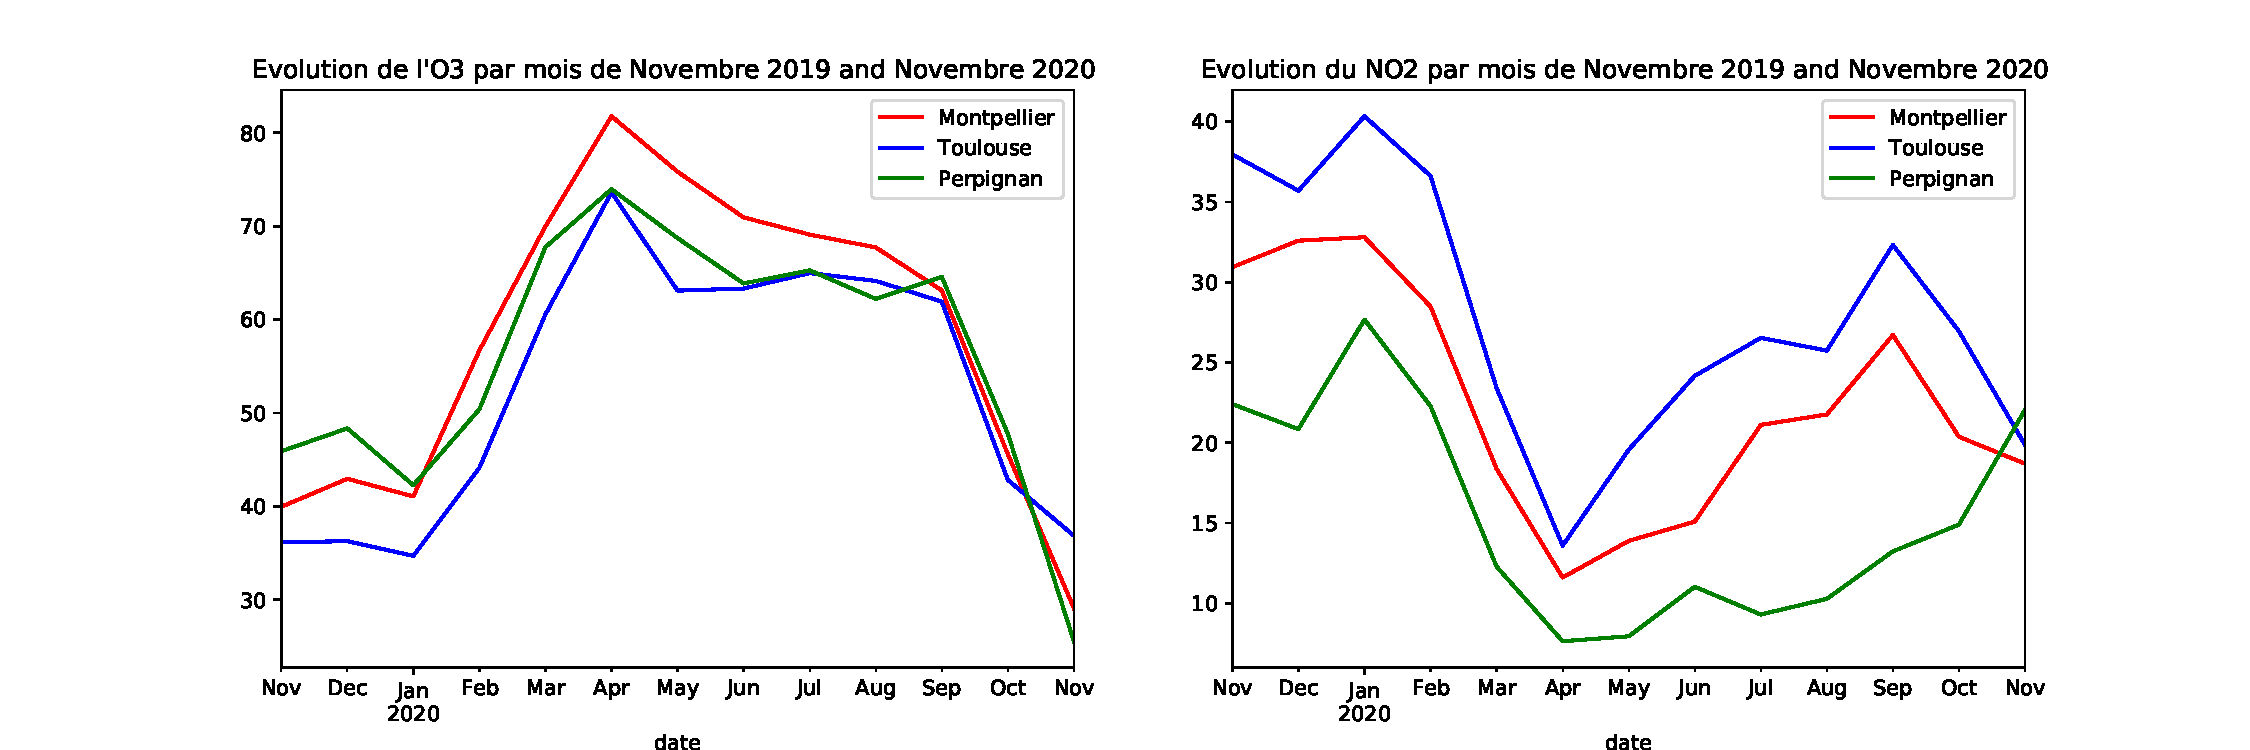
\includegraphics[width=\textwidth]{Evolution_O3_NO2.pdf}
  \caption[Titre plus synthétique aller voir comme il diffère du titre
  original.]{gauche: Evolution de l'ozone (O3) pour Montpellier, Toulouse et Perpignan l'année 2020. Droite: l'évolution du dioxyde d'azote (NO2) pour 3 même villes.  }
  \label{fig:Evo}
\end{figure}

%%%%%%%%%%%%%%%%%%%%%%%%%%%%%%%%%%%%%%%%%%%%%%%%%%%%%%%%%%%%%%%%%%%%%%%%
%%                                                                    %%
%%                          ANOVA                                     %%
%%                                                                    %%
%%%%%%%%%%%%%%%%%%%%%%%%%%%%%%%%%%%%%%%%%%%%%%%%%%%%%%%%%%%%%%%%%%%%%%%%

\chapter{Anova sur les niveaux de pollutions}
\label{cha:Anova}

Nous allons maintenant réaliser un test Anova pour comparer les moyennes de différentes villes de notre de base et voir s'il y a, ou non, une différence entre elles. Nous avons choisi deux cas de figures. Le premier cas, nous avons choisi de prendre des villes assez proche géographiquement de Montpellier ( comme Lattes par exemple). Le deuxième cas, sur des villes éloignés de Montpellier ( comme Toulouse ).

Le modèle :  \[y_{ij}=\mu^*+ \alpha_j+\varepsilon_{ij}\]\\
$i$ : taille de la période étudiée
$j$  nombre de villes \\





\section{Comparaison entre 3 villes éloignés}
\label{sec:Comparaison entre  3 villes éloignés}

nous allons tester l hypothèse  $H_0 :'\mu_{Montpellier}=\mu_{Toulouse}=\mu_{Perpignan}$ avec $\alpha=0.05$\\


\subsection{Durant l'année 2020}
\label{sec:Durant l'année 2020}

Nous appliquons notre modèle à toute la base pour nos trois villes: 
Grace au diagramme de probabilité des résidues, nous constatons que les résidus suivent bien une distribution normale \\

Nous avons l hypothèse  $H_0 :'\mu_{Montpellier}=\mu_{Toulouse}=\mu_{Perpignan}$ et $\alpha=0.05$\\

Dans le tableau~\ref{tab:anovmtpy}, page~\pageref{tab:anovmtpy} nous lisons que la $p_{value} = 0.01$ est plus petite que $\alpha$ alors on rejette $H_0$  et il y a donc une différences significative du niveau moyen d'Ozone entre Montpellier Toulouse et Perpignan


\subsection{Pendant le confinement}
\label{sec:pendant le confinement }

Nous appliquons maintenant notre modèle aux dates du confinement nos trois villes: 


Nous avons l hypothèse  $H_0 :'\mu_{Montpellier}=\mu_{Toulouse}=\mu_{Perpignan}$ et $\alpha=0.05$\\

Dans le tableau~\ref{tab:anovmtp}, page~\pageref{tab:anovmtp} nous lisons que la $p_{value} = 0.01$ est plus petite que $\alpha$ alors on rejette $H_0$  et il y a donc une différences significative du niveau moyen d'Ozone entre Montpellier Toulouse et Perpignan



\section{Comparaison entre 3 villes proche}
\label{sec:Comparaison entre 3 villes proche}





\subsection{Durant l'année 2020}
\label{sec:Durant l'année 2020}


Dans le tableau~\ref{tab:anovmgly}, page~\pageref{tab:anovmgly} nous lisons que la $p_{value}$  est plus petite que $\alpha$ alors on rejette $H_0$  et il y a donc une différences significative du niveau moyen d'Ozone entre Montpellier, Saint-Gély-du-fesc et Lattes durant l'année écoulé

\subsection{Pendant le confinement}
\label{sec:pendant le confinement }

Dans le tableau~\ref{tab:anovmgl}, page~\pageref{tab:anovmgl} nous lisons que la $p_{value}$  est plus petite que $\alpha$ alors on rejette $H_0$  et il y a donc une différences significative du niveau moyen d'Ozone entre Montpellier, Saint-Gély-du-fesc et Lattes pendant le confinenment

%%%%%%%%%%%%%%%%%%%%%%%%%%%%%%%%%%%%%%%%%%%%%%%%%%%%%%%%%%%%%%%%%%%%%%%%
%%                                                                    %%
%%                      Tableaux Anova                                %%
%%                                                                    %%
%%%%%%%%%%%%%%%%%%%%%%%%%%%%%%%%%%%%%%%%%%%%%%%%%%%%%%%%%%%%%%%%%%%%%%%%



\begin{table}
  \centering
  \caption[]{Table de l'Anova réalisé sur Montpellier, Toulouse et Perpignan pour ce qui
  concerne l'Ozone sur une année .}
  \label{tab:anovmtpy}
  \begin{tabular}{lcccc}
    \hline
    & \multicolumn{4}{c}{Table Anova}\\
    & $\text{sum squared}$ & $\text{df}$ & $\text{F}$ & $\text{Pr(>F)}$ \\
    \hline
    \text{nom com} & 2529.04 & 2 & 3.19 & 0.0412\\
    \text{Residual} & 418751.49 & 1059 & NaN  & NaN  \\
    \hline
  \end{tabular}
\end{table}
%% table2
\begin{table}
  \centering
  \caption[]{Table de l'Anova réalisé sur Montpellier, Toulouse et Perpignan pour ce qui
  concerne l'Ozone pendant le confinement .}
  \label{tab:anovmtp}
  \begin{tabular}{lcccc}
    \hline
    & \multicolumn{4}{c}{Table Anova}\\
    & $\text{sum squared}$ & $\text{df}$ & $\text{F}$ & $\text{Pr(>F)}$ \\
    \hline
    \text{nom com} & 2361.63 & 2 & 4.6 & 0.01\\
    \text{Residual} & 69304.51 & 270 & NaN  & NaN  \\
    \hline
  \end{tabular}
\end{table}
%% tazble3: ville proche + année

\begin{table}
  \centering
  \caption[]{Table de l'Anova réalisé sur Montpellier, Saint-Gély-du-fesc et Lattes pour ce qui
  concerne l'Ozone  sur une année .}
  \label{tab:anovmgly}
  \begin{tabular}{lcccc}
    \hline
    & \multicolumn{4}{c}{Table Anova}\\
    & $\text{sum squared}$ & $\text{df}$ & $\text{F}$ & $\text{Pr(>F)}$ \\
    \hline
    \text{nom com} & 9212.287 & 2 & 11.93& $ >10^{-5}$\\
    \text{Residual} & 416955.05 & 1080 & NaN  & NaN  \\
    \hline
  \end{tabular}
\end{table}
 %ù table 4 ville proche confinement
 \begin{table}
  \centering
  \caption[]{Table de l'Anova réalisé sur Montpellier, Saint-Gély-du-fesc et Lattes pour ce qui
  concerne l'Ozone pendant le confinement .}
  \label{tab:anovmgl}
  \begin{tabular}{lcccc}
    \hline
    & \multicolumn{4}{c}{Table Anova}\\
    & $\text{sum squared}$ & $\text{df}$ & $\text{F}$ & $\text{Pr(>F)}$ \\
    \hline
    \text{nom com} & 3616.09 & 2 & 7.145 & $9.4*10^{-4}$\\
    \text{Residual} & 68824.766 & 272 & NaN  & NaN  \\
    \hline
  \end{tabular}
\end{table}



%%%%%%%%%%%%%%%%%%%%%%%%%%%%%%%%%%%%%%%%%%%%%%%%%%%%%%%%%%%%%%%%%%%%%%%%
%%                                                                    %%
%%                      CONCLUSION                                    %%
%%                                                                    %%
%%%%%%%%%%%%%%%%%%%%%%%%%%%%%%%%%%%%%%%%%%%%%%%%%%%%%%%%%%%%%%%%%%%%%%%%

\chapter*{Conclusion}

Lors de nos différentes études nous avons pu constater une différence sur cette année du niveau de pollution suivant les villes étudiées. Nous auront pu penser  ne pas observer de différence que pour ce qui est des villes proches ( Montpellier, Saint Gély , Lattes ).


\nocite{R,Dav,Agr,nat,Li:1985,BrCl,CM,LesSpi,LitRub,MCN}
\bibliographystyle{apalike}  
\bibliography{references}

\end{document}
